\documentclass[11pt]{article}
\usepackage{hyperref}
\usepackage{amsthm}
\usepackage{amsmath}
\usepackage{amsfonts}
\usepackage{tikz}
\usepackage{ wasysym }

\newtheorem{example}{Example}


\author{}
\title{}

\begin{document}
%\maketitle
{\Large
Change Document name to: Graded Homework 1\_Jacob\_Nicholas
\noindent NAME:  Nicholas Jacob\\ 
STUDENT ID: \# 113578513\\
GRADED HOMEWORK NUMBER: 1\\
COURSE: CS/DSA 4513 DATABASE MANAGEMENT\\ 
SECTION: ONLINE\\SEMESTER: FALL 2023\\
INSTRUCTOR:  DR. LE GRUENWALD\\
 SCORE:}

\newpage
\begin{enumerate}
\item ChatGPT conversation can be found in the link  \url{https://chat.openai.com/share/0e84b965-4e65-405c-a45e-fa333c293a4d}

Here is the first prompt and result of my conversation:

\begin{quotation}
\noindent Me

Can you describe a aggregation in an ER diagram


\noindent ChatGPT

In an Entity-Relationship (ER) diagram, aggregation is a type of relationship that represents a whole-part relationship between two entities. It is used to model scenarios where one entity is composed of or is made up of other entities. Aggregation is a conceptual modeling concept used to show how smaller, related entities combine to form a larger, more complex entity.

Here are some key points to understand about aggregation in an ER diagram:

    Diamond-shaped notation: In ER diagrams, aggregation is typically represented using a diamond-shaped symbol. The diamond shape is placed next to the entity that represents the whole or the container, and a line is drawn from the diamond to the entities that represent the parts or components.

    Whole-Part Relationship: Aggregation signifies a relationship where one entity (the whole) is composed of or contains other entities (the parts). This relationship indicates that the parts are conceptually dependent on the existence of the whole.

    Optional or Mandatory: Aggregation relationships can be optional or mandatory. In other words, the parts may or may not exist without the whole. In some cases, the existence of parts is mandatory (strong aggregation), while in others, it may be optional (weak aggregation).

    Cardinality: Aggregation relationships can have cardinality constraints, indicating how many parts are associated with a single whole and vice versa. Cardinality constraints are usually represented near the ends of the lines connecting the diamond to the entities.

Here's a simple example to illustrate aggregation in an ER diagram:

Consider a library management system:

    The "Library" entity represents the whole, and it has an aggregation relationship with the "Book" entity, which represents the parts.
    The aggregation diamond would be placed next to the "Library" entity, and a line would connect it to the "Book" entity.
    If the aggregation is optional, it would mean that a library may or may not have books (0..* on the "Book" side), and a book must belong to a library (1 on the "Library" side).

In this example, the aggregation relationship shows that a library is composed of books, but a book can exist independently of a specific library. It helps in modeling the structural relationship between libraries and books within the system.

Remember that aggregation is just one of several types of relationships you can use in an ER diagram to model different aspects of your data and its structure. Other common relationships include associations, generalization/specialization (inheritance), and many-to-many relationships, among others.
    
\end{quotation}

We see right away that ChatGPT is getting close to the textbook definition.  The whole-part idea was not what was presented in the textbook, rather it is a simplification of the idea of the abstraction which the text and instructor prefer.  I find this whole-part idea a nice way to clarify this definition but in someways abstraction is superior.  These might include the idea of multiple relations and entities being combined.  With whole-part it is not clear that you could do this.

The usage here is not so clear.  We don't see the idea of boxing the whole and identifying it as a new abstracted identity.  ChatGPT does not clearly explain how you would make the abstraction work in an ER diagram even though it attempts to with the discussion of diamonds for the relationships.

The example here is very poor.  Library and books is really just talking about a one-to-many relationship of ``has".  This may partially be because they are talking about a many branch system but in any case the extra layer of abstraction provided by aggregation is unnecessary in this example.  

While I didn't include it here (see link above for full conversation), I kept asking chatGPT if it could improve on this answer involving usage and examples.  It did clarify the usage in one of many bullet points but several of the bullets were erroneously being called aggregation.  It did not provide a strong example of aggregation when directly asked.  Again using many-to-one relationships.

Overall I am disappointed in this answer but not surprised as I am seeing chatGPT text in my work regularly and can often spot it right away by the language used and the simplification mistakes to the broader topic.

\item ER Diagram:  Highlights of my approach are aggregation of booking entity, specialization of person to host and/or guest and referral aggregation with a weak relationship tied to booking for earning of referral bonus.

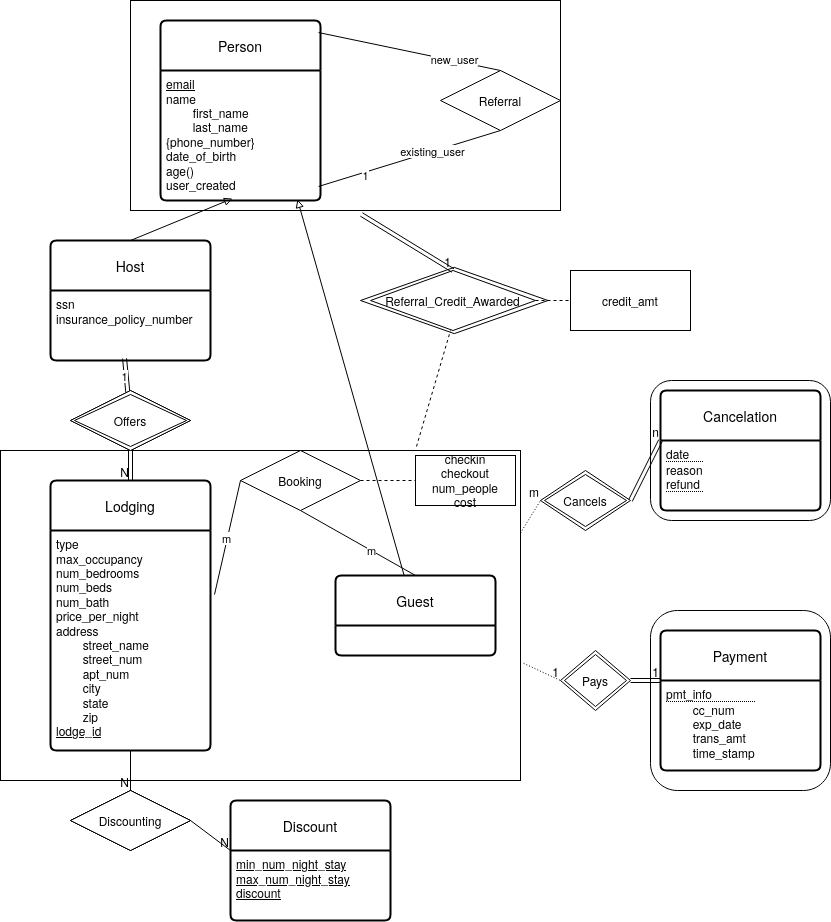
\includegraphics[width = \textwidth]{question1.png}

\item Yes this relationship could be created.  Add a relationship between guest and lodging outside of the aggregation represented by booking.  It might be best practice to not let guests review lodgings they have not booked.  If that was the case, you'd link the aggregation to reviews.  The review will need its own entity entitled Reviews. I have done so below and added the attributes for review.  I do not consider this as a weak entity due to the fact that reviews should be shared without guest info and removed from lodgings if found erroneous.

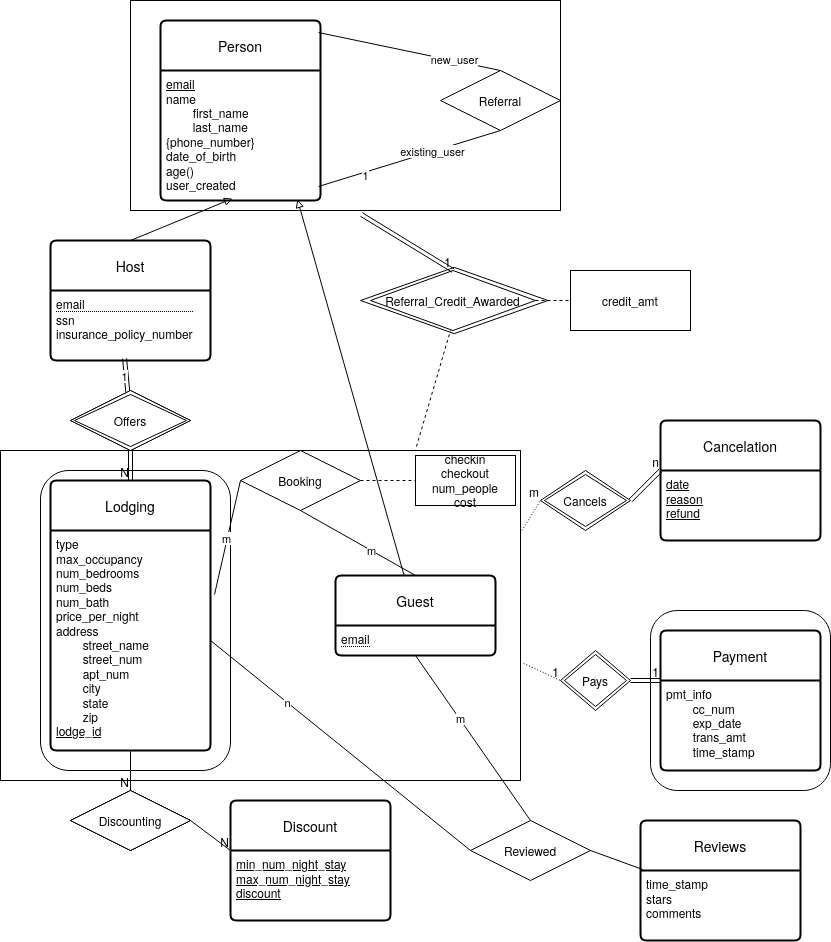
\includegraphics[width = \textwidth]{question3.png}

\item You could also make a new weak entity and weak relationship that was bank and banks\_with and include all the information there.  Membership will be required (both ways since Hosts will need a banking account and banking accounts will need hosts).  I have added the required in not the best fashion below.

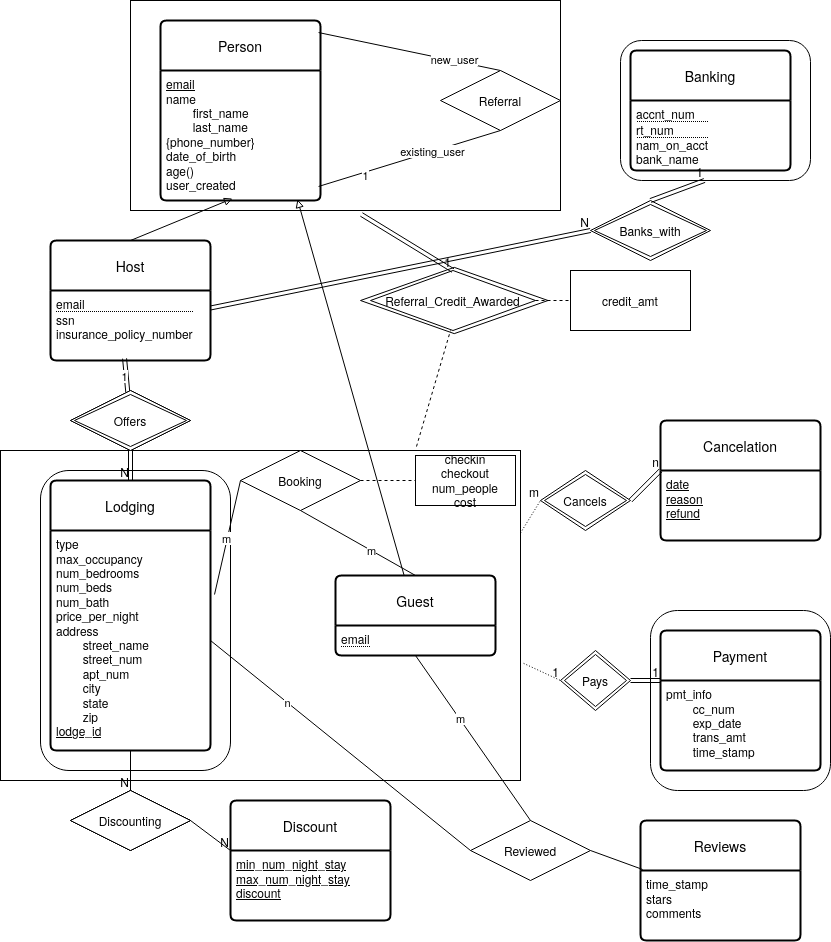
\includegraphics[width = \textwidth]{question4.png}

After considering this question for a bit, you could also add the banking information as an attribute.  It would possibly be multi-valued but it could be add just to the host entity rather than mucking up the tree.



\end{enumerate}



\end{document}